\documentclass{article}
\usepackage{amsmath}
\usepackage{graphicx}
\usepackage{ntheorem}
\newtheorem{theorem}{Theorem}[section]
\newtheorem{corollary}{Corollary}[theorem]
\newtheorem{lemma}[theorem]{Lemma}
\usepackage{tkz-graph}
\usetikzlibrary{arrows}
\usetikzlibrary{shapes.geometric}
\usepackage{hyperref}


\SetVertexNormal[Shape      = circle,
                 FillColor  = cyan,
                 LineWidth  = 2pt]
\SetUpEdge[lw         = 1pt,
           color      = black,
           labelcolor = white,
           labeltext  = red,
           labelstyle = {sloped,draw,text=blue}]
\tikzset{Bullet/.style={fill=black,draw,color=#1,circle,minimum size=3pt,scale=0.75}}


\begin{document}


\title{Causal Inference with Graphical Neural Networks}
\author{Gwen Johnson\and Dylan Skinner\and Dallin Stewart\and Jason Vasquez}
\date{\today}
\maketitle

\section{Introduction}
\label{intro}


\section{Graph Neural Networks}
\label{gnn}

Originally proposed in 2005 by Mori et al.~\cite{gori2005new}, Graph Neural Networks 
(GNNs) are a class of neural networks that operate on graph-structured data. 
They have gained significant attention in recent years due to their versatility 
in handling various types of graph data, including social networks, citation networks, 
biological networks, and more. 

Unlike traditional neural networks, which operate on 
grid-like structures such as images or sequences, GNNs are specifically designed to 
capture and leverage the structural information present in graphs. One of their 
key strengths lies in their ability to learn meaningful representations of nodes in a 
graph, which can then be used for various downstream tasks such as node classification, 
link prediction, and graph classification. Their ability to capture and model complex 
relationships in graph data makes them invaluable tools for exploring and understanding 
real-world phenomena represented in graph form.

In our project, we are utilizing the power of GNNs to perform a supervised classification
task. This means we are training a GNN on a labeled, tabular dataset, where each graph instance
(or node) is associated with a target label.


% Introduce the topic of causal inference with Graphical Neural Networks (GNNs).

\section{$\textbf{do}$ Operator}
\label{do}

The \textbf{do} operator is a way to represent interventions in a causal model. 
It is a way to represent the effect of an intervention on a variable. As an example, 
consider the following model involving smoking.

If a person's fingernails $(N)$ have turned yellow, this implies a higher probability 
that they are a heavy smoker $(S)$ and hence have a higher probability of developing 
lung cancer $(C)$. But, simply dyeing a persons fingernails yellow does not impact 
their probability of developing lung cancer. 

So, in terms of $\textbf{do}$ calculus, we can denote the process of setting a 
variable $N$ to have a value $\textit{yellow}$ by $\textbf{do}(N = \textit{yellow})$. 
We note that 

\begin{equation*}
P(C \;|\;N = \textit{yellow}) \neq P(C\;|\; \textbf{do}(N=\textit{yellow})).
\end{equation*}

With this in mind, we now define the $\textbf{do}$ operator.

\begin{theorem}[{{\cite{pearl2009causal}}}]
    In a causal diagram $\Gamma$ with nodes $X_1,\dots, X_n$ and joint distribution 
    $P(X_1, \dots, X_n)$, the result of doing $X_i = x_i$ on the joint distribution is

    \[
        P(X_1, \dots, X_n \;|\; \textbf{do}(X_i = x_i)) = \frac{P(x_1,\dots,x_n)}{P(x_i\;|\; \textup{par}(x_i))} = \prod_{j\neq i}P(x_j\;|\; \textup{par}(x_j)).
    \]
    \label{theorem:do}
\end{theorem}

In this, we have $\text{par}(x_i)$ represent values of the parent nodes of $\text{PAR}(X_i)$ of $X_i$ in $\Gamma$.
The probabilities on the right hand side of the above equation are what we call \textit{preintervention}. 
This means they use the original probabilities from the original model before doing $X_i = x_i$.

It is important to note that the above equation is how we calculate the probability of several events 
happening given one event has happened. What if we want to get the probability of a single event happening, 
given we do a single event? That leads to the following corollary.

\begin{corollary}
    If $X$ and $Y$ are random variables in a causal diagram $\Gamma$ and $\textup{PAR}(X)$ are the parents of $X$, then

    \[P(y\;|\;  \textbf{do}(x)) = \sum_{\textup{par}}\frac{P(x,\,y,\,\textup{par})}{P(x\;|\; \textup{par})},\]

    where the sum runs over all values $\textup{par}$ that the variables $\textup{PAR}(X)$ can take. If $X$ has no parents, then

    \[P(y\;|\; \textbf{do}(x)) = \frac{P(x,\,y)}{P(x)} = P(y\;|\; x).\]
    \label{corollary:do}
\end{corollary}

Let us now consider a basic example to see how this works. Consider the following causal diagram in Figure~\ref{fig:causal_dia}.

\begin{figure}[h]
    \centering
    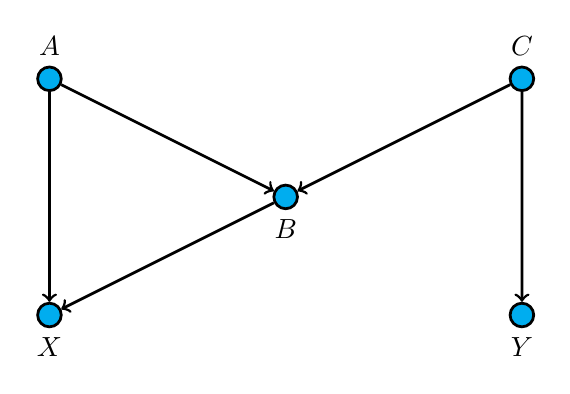
\begin{tikzpicture}[scale=1.5, Bullet/.style={circle, draw=black, fill=#1, inner sep=0pt, minimum size=3mm, line width=1.pt}]
        \node[Bullet=cyan,label=above :{$A$}] (A) at (0,2){};
        \node[Bullet=cyan,label=above :{$C$}] (C) at (4,2){};
        \node[Bullet=cyan,label=below :{$B$}] (B) at (2,1){};
        \node[Bullet=cyan,label=below :{$Y$}] (Y) at (4,0){};
        \node[Bullet=cyan,label=below :{$X$}] (X) at (0,0){};
    
        \draw[->, line width=1] (A) -- (B);
        \draw[->, line width=1] (C) -- (B);
        \draw[->, line width=1] (B) -- (X);
        \draw[->, line width=1] (C) -- (Y);
        \draw[->, line width=1] (A) -- (X);
    \end{tikzpicture}
    \caption{Basic causal diagram. Note it is in the form of a directed acyclic graph (DAG).}
    \label{fig:causal_dia}
\end{figure}

In this diagram, we can see that $A$ and $C$ are both parents of $B$. So, for any values of $x$ and $b$, 
Corollary~\ref{corollary:do} tells us that

\begin{align*}
    P(X = x \,|\, \textbf{do}(B=b)) &= \sum_{\text{par}(b)}\frac{P(x, \,b, \,\text{par}(b))}{P(b\,|\, \text{par}(b))} \\
    %  &= \sum_{a}\sum_{c}\frac{P(X=x\,, \, A=a\,,\, B=b \, ,\, C=c)}{P(B=b \;|\; A=a,\, C=c)} \\
    %  &= \sum_{a}\sum_{c}\frac{P(X=x\;|\; A=a\,,\, B=b)P(B=b\;|\; A=a,\, C=c)P(A=a)P(C=c)}{P(B=b \;|\; A=a,\, C=c)} \\
    %  &= \sum_{a}\sum_{c}P(X=x\;|\; A=a\,,\, B=b)P(A=a)P(C=c) \\
\end{align*}

which, written out, is 

\begin{equation*}
    \sum_{\text{par}(b)}\frac{P(x, \,b, \,\text{par}(b))}{P(b\,|\, \text{par}(b))} = \sum_{a}\sum_{c}\frac{P(X=x\,, \, A=a\,,\, B=b \, ,\, C=c)}{P(B=b \;|\; A=a,\, C=c)}.
\end{equation*}

By dependence of nodes only on their parents and the rules of probability, this turns into

\begin{equation*}
    \sum_{a}\sum_{c}\frac{P(X=x\;|\; A=a\,,\, B=b)P(B=b\;|\; A=a,\, C=c)P(A=a)P(C=c)}{P(B=b \;|\; A=a,\, C=c)},
\end{equation*}

which simplifies to

\begin{equation*}
    \sum_{a}\sum_{c}P(X=x\;|\; A=a\,,\, B=b)P(A=a)P(C=c).
\end{equation*}

Since there is only one instance where we are considering the probability with respect to $c$, 
we can simplify this to

\begin{equation*}
    \sum_{a}P(X=x\;|\; A=a\,,\, B=b)P(A=a),
\end{equation*}

which is our final answer.

While this introduction to the \textbf{do} operator might feel a bit abstract, it is the foundation
of all current research in causal inference. 





\section{Data}
\label{data}

For our project, we used the LUCAS0 dataset~\cite{lucas_dataset}, which is a toy data set 
generated artificially by causal Bayesian networks with binary variables. The LUCAS0 dataset
is a DAG with 11 nodes and 2000 training samples, where the DAG is represented as in Figure~\ref{fig:lucas_dag}.

\begin{figure}[h]
    \centering
    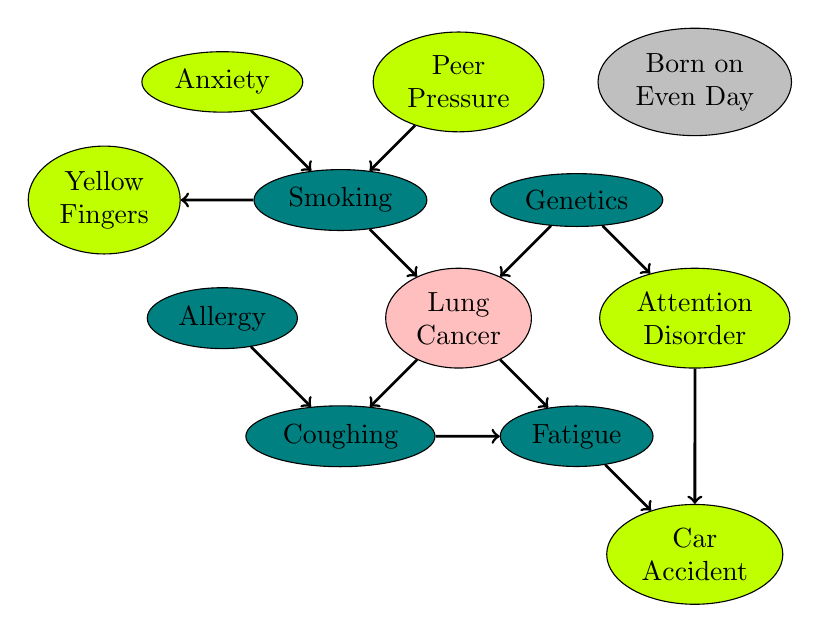
\begin{tikzpicture}[scale=1.5, Bullet/.style={circle, draw=black, fill=#1, inner sep=0pt, minimum size=3mm, line width=1.pt}]
        % \draw[help lines, gray] (0,0) grid (6,6);
        \node[ellipse, draw=black, fill=lime] (A) at (2,2){Anxiety};
        \node[ellipse, draw=black, fill=lime, align=center] (P) at (4,2){Peer\\Pressure};
        \node[ellipse, draw=black, fill=teal] (S) at (3,1){Smoking};
        \node[ellipse, draw=black, fill=lime, align=center] (Y) at (1,1){Yellow\\Fingers};
        \node[ellipse, draw=black, fill=lightgray, align=center] (B) at (6, 2){Born on\\Even Day};
        \node[ellipse, draw=black, fill=teal, align=center] (G) at (5, 1){Genetics};
        \node[ellipse, draw=black, fill=teal, align=center] (Al) at (2, 0){Allergy};
        \node[ellipse, draw=black, fill=pink, align=center] (L) at (4, 0){Lung\\Cancer};
        \node[ellipse, draw=black, fill=lime, align=center] (AD) at (6, 0){Attention\\Disorder};
        \node[ellipse, draw=black, fill=teal, align=center] (C) at (3, -1){Coughing};
        \node[ellipse, draw=black, fill=teal, align=center] (F) at (5, -1){Fatigue};
        \node[ellipse, draw=black, fill=lime, align=center] (CA) at (6, -2){Car\\Accident};
    
        \draw[->, line width=1] (A) -- (S);
        \draw[->, line width=1] (P) -- (S);
        \draw[->, line width=1] (S) -- (Y);
        \draw[->, line width=1] (S) -- (L);
        \draw[->, line width=1] (G) -- (L);
        \draw[->, line width=1] (G) -- (AD);
        \draw[->, line width=1] (Al) -- (C);
        \draw[->, line width=1] (L) -- (C);
        \draw[->, line width=1] (L) -- (F);
        \draw[->, line width=1] (C) -- (F);
        \draw[->, line width=1] (F) -- (CA);
        \draw[->, line width=1] (AD) -- (CA);

    \end{tikzpicture}
    \caption{Basic causal diagram. Note it is in the form of a directed acyclic graph (DAG). Our target variable
    is shaded in ${\color{pink} \textbf{pink}}$, and the nodes in {\color{teal} \textbf{teal}} constitude the Markov
    blanket of the target variable.}
    \label{fig:lucas_dag}
\end{figure}

Each node of the graph was is associated with a specific conditional probability that the
creators of the dataset used to generate the data. These probabilities can be found in Table~\ref{tab:lucas_probs}
in Appendix~\ref{create}.


\section{do Calculus Result stuff (idk where this goes)}

Let's consider the following conditional probabilities with \textbf{do} operators applied:

\begin{align*}
    P(\text{LC} = \text{T} \;&|\; \textbf{do}(\text{YF} = \text{T})), \\
    P(\text{LC} = \text{T} \;&|\; \textbf{do}(\text{PP} = \text{T})), \\
    P(\text{LC} = \text{T} \;&|\; \textbf{do}(\text{A} = \text{T})), \\
    P(\text{LC} = \text{T} \;&|\; \textbf{do}(\text{AD} = \text{T})), \\
    P(\text{LC} = \text{T} \;&|\; \textbf{do}(\text{CA} = \text{T})), \\
\end{align*}

where LC is lung cancer, YF is yellow fingers, PP is peer pressure, A is anxiety, AD is attention disorder, and CA 
is car accident. We note that we chose this probability because it does not involve any
variables that are in the Markov blanket of our target variable. Thus, we should expect that there is very little
predictive power in this probability.

Plugging forward with \textbf{do} calculus, we can write $P(\text{LC} = \text{T} \;|\; \textbf{do}(\text{YF} = \text{T}))$ as
(using corollary~\ref{corollary:do})

\begin{equation*}
    P(\text{LC} = \text{T} \;|\; \textbf{do}(\text{YF} = \text{T})) = 
    \sum_{s\in\{T, F\}} \frac{P(\text{YF} = \text{T},\, \text{LC} = \text{T},\, \text{S} = s)}{P(\text{YF} = \text{T}\,|\, \text{S} = s)},
\end{equation*}

where $\text{S}$ is smoking. Using the property that we can split the numerator into probabilities only involving parents ({\color{red}rewrite})

\begin{equation*}
    \sum_{s\in\{T, F\}}\frac{P(\text{YF} =\text{T}\;|\; \text{S} = s) P(\text{LC} 
    = \text{T}\;|\; \text{S}=s,\, \text{G}) P(\text{S}=s\;|\;\text{A},\, \text{PP})}
    {P(\text{YF} = \text{T}\;|\; \text{S} = s)}.
\end{equation*}

All of these fun conditionals lead us to

\begin{equation*}
    \sum_{s,a,g,p}\frac{P(\text{YF} =\text{T}\;|\; \text{S} = s) P(\text{LC} 
    = \text{T}\;|\; \text{S}=s,\, \text{G}=g) P(\text{S}=s\;|\;\text{A}=a,\, \text{PP}=p)}
    {P(\text{YF} = \text{T}\;|\; \text{S} = s)},
\end{equation*}

where each $s,a,g,p$ is summed over the set $\{T, F\}$.

% Provide background information on causal inference, neural networks, and Graphical Neural Networks (GNNs).

\section{Methodology}

% Describe the methodology of using GNNs for causal inference. Include information on how GNNs are trained, how causal inference is performed, etc.

\section{Experiments}

% Present the experiments conducted to evaluate the performance of GNNs for causal inference. Include dataset descriptions, experimental setup, and results.

\subsection{Dataset Description}

% Describe the datasets used in the experiments.

\subsection{Experimental Setup}

% Explain the experimental setup, including model architecture, training procedure, hyperparameters, etc.

\subsection{Results}

% Present and analyze the results of the experiments. Include metrics, comparisons with baseline methods, and any insights gained.

\section{Discussion}

% Discuss the implications of the results, limitations of the approach, potential future research directions, etc.

\section{Conclusion}

% Summarize the key findings of the study and conclude the paper.

\section*{Acknowledgments}

% Acknowledge any individuals or organizations that contributed to the project.


\newpage
% Bibliography
\bibliographystyle{plain}
\bibliography{references} % Replace 'references' with the name of your .bib file

\newpage

\section*{Appendix}

\appendix
\section{Creating the LUCAS0 Dataset}
\label{create}

As described in the \nameref{data} section, the LUCAS0 dataset is a toy dataset generated 
artificially by causal Bayesian networks with binary variables. The dataset consists of 
11 nodes and 2000 training samples. The causal diagram for the LUCAS0 dataset is shown in Figure~\ref{fig:lucas_dag}.

On the website, the authors mention that each node of the graph is associated with conditional probabilities
which were used to generate the data. These probabilities are found in Table~\ref{tab:lucas_probs}.

\begin{table}[h]
    \centering
    \begin{tabular}{|c|c|}
        \hline
        \multicolumn{2}{|c|}{\textbf{Conditional Probabilities}} \\
        \hline
        \textit{Conditional} & \textit{Probability} \\
        \hline
        P(Anxiety=T) & 0.64277 \\ \hline
        P(Peer Pressure=T) & 0.32997 \\ \hline
        P(Smoking=T $\vert$ Peer Pressure=F, Anxiety=F) & 0.43118 \\ \hline
        P(Smoking=T $\vert$ Peer Pressure=T, Anxiety=F) & 0.74591 \\ \hline
        P(Smoking=T $\vert$ Peer Pressure=F, Anxiety=T) & 0.8686 \\ \hline
        P(Smoking=T $\vert$ Peer Pressure=T, Anxiety=T) & 0.91576 \\ \hline
        P(Yellow Fingers=T $\vert$ Smoking=F) & 0.23119 \\ \hline
        P(Yellow Fingers=T $\vert$ Smoking=T) & 0.95372 \\ \hline
        P(Genetics=T) & 0.15953 \\ \hline
        P(Lung cancer=T $\vert$ Genetics=F, Smoking=F) & 0.23146 \\ \hline
        P(Lung cancer=T $\vert$ Genetics=T, Smoking=F) & 0.86996 \\ \hline
        P(Lung cancer=T $\vert$ Genetics=F, Smoking=T) & 0.83934 \\ \hline
        P(Lung cancer=T $\vert$ Genetics=T, Smoking=T) & 0.99351 \\ \hline
        P(Attention Disorder=T $\vert$ Genetics=F) & 0.28956 \\ \hline
        P(Attention Disorder=T $\vert$ Genetics=T) & 0.68706 \\ \hline
        P(Born an Even Day=T) & 0.5 \\ \hline
        P(Allergy=T) & 0.32841 \\ \hline
        P(Coughing=T $\vert$ Allergy=F, Lung cancer=F) & 0.1347 \\ \hline
        P(Coughing=T $\vert$ Allergy=T, Lung cancer=F) & 0.64592 \\ \hline
        P(Coughing=T $\vert$ Allergy=F, Lung cancer=T) & 0.7664 \\ \hline
        P(Coughing=T $\vert$ Allergy=T, Lung cancer=T) & 0.99947 \\ \hline
        P(Fatigue=T $\vert$ Lung cancer=F, Coughing=F) & 0.35212 \\ \hline
        P(Fatigue=T $\vert$ Lung cancer=T, Coughing=F) & 0.56514 \\ \hline
        P(Fatigue=T $\vert$ Lung cancer=F, Coughing=T) & 0.80016 \\ \hline
        P(Fatigue=T $\vert$ Lung cancer=T, Coughing=T) & 0.89589 \\ \hline
        P(Car Accident=T $\vert$ Attention Disorder=F, Fatigue=F) & 0.2274 \\ \hline
        P(Car Accident=T $\vert$ Attention Disorder=T, Fatigue=F) & 0.779 \\ \hline
        P(Car Accident=T $\vert$ Attention Disorder=F, Fatigue=T) & 0.78861 \\ \hline
        P(Car Accident=T $\vert$ Attention Disorder=T, Fatigue=T) & 0.97169 \\ \hline
        \hline
    \end{tabular}
    \caption{Conditional probabilities for the nodes in the LUCAS0 dataset.}
    \label{tab:lucas_probs}
\end{table}







\end{document}
